Validators derived in this approach can be proven sound and complete:
\[\begin{array}{r@{\;}l}
\forall p:\Prog,&\letin{s}{\serverOf(p)}\\
&\letin{v}{\validatorOf(p)}\\
&\rejSound v s\wedge\rejComplete v s\\
&\text{\it i.e. }\forall t:\List(Q\times A),\\
&\qquad\valid s t\iff\accepts v t\\
&\qquad\text{\it i.e. }\exists s',\behaves s t s'\iff\exists v',\behaves v t v'
\end{array}\]

In this subsection, I first present a generic framework for proving validators'
correctness properties, and then demonstrate its usage by applying it to
$\Prog$-based validators.

The ``equivalence between server production and validator consumption of all
traces'' is proven by introducing a loop invariant.  The invariant is a
bisimulation between the server and the validator, which is preserved for each
step of the trace produced/consumed.

\subsection{Proving rejection soundness}
The proof of ``any trace produceable by the server is consumable by the
validator'' is by forward induction on the server's execution path.  The
corresponding validation path is constructed based on the following hypotheses:
\begin{enumerate}
\item The initial server state reflects the initial validator state:
  \begin{equation}
    \tag{RejSound1}
    \label{eq:rs1}
    \Reflects{(v_0:V)}{(s_0:S)}
  \end{equation}
\item Any server step whose pre-execution state reflects some pre-validation
  state can be consumed by the validator into a post-validation state that
  reflects the post-execution state:
  \begin{align*}
    &\forall(q:Q)(c:C)(a:A)(s,s':S)(v:V),\\
    &\sstep(q,c,s)=(a,s')\wedge\Reflects{v}{s}\\
    \tag{RejSound2}
    \label{eq:rs2}
    &\implies\exists v':V,\vstep(q,a,v)=\Some{v'}\wedge\Reflects{v'}{s'}
  \end{align*}
  \begin{center}
    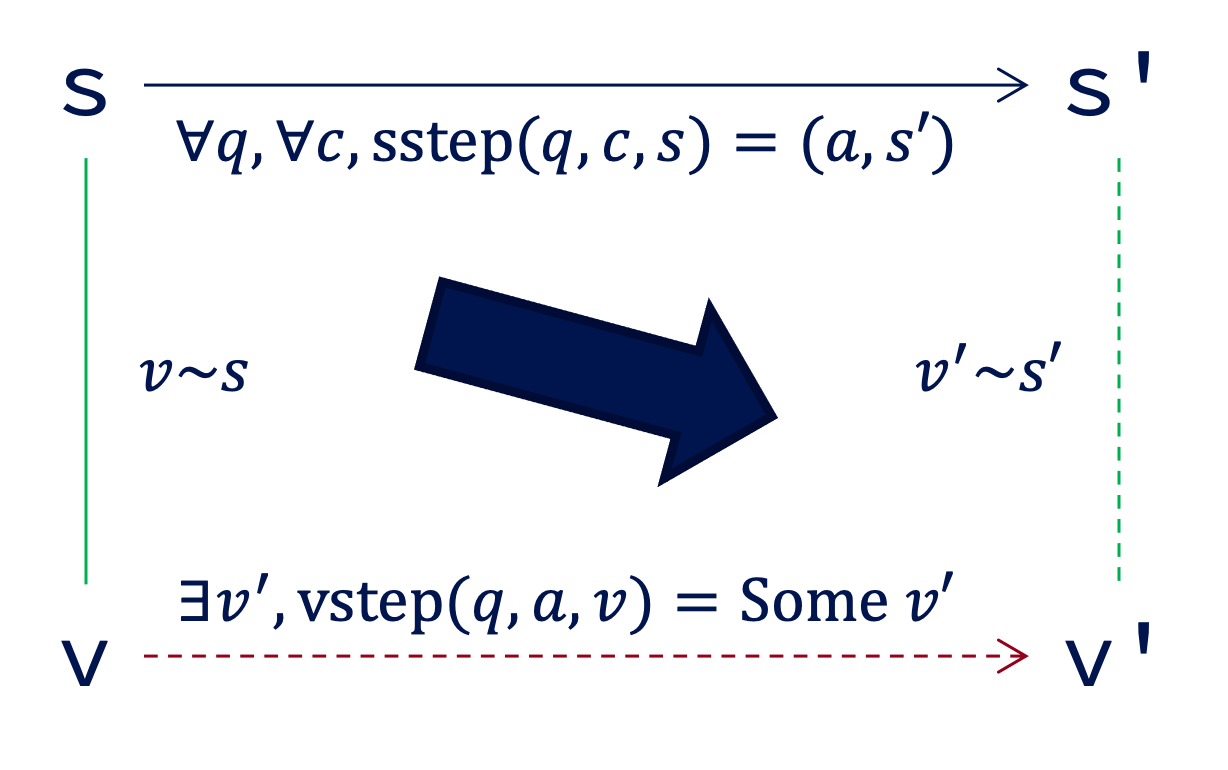
\includegraphics[width=.5\textwidth]{figures/sound}
  \end{center}
\end{enumerate}

\subsection{Proving rejection completeness}
The proof of ``any trace consumable by the validator is produceable by the
server'' is by backward induction on the validator's execution path.  The
corresponding server path is constructed based on the following hypotheses:

\begin{enumerate}
\item Any accepting validator step has some server state that reflects the
  post-validation state:
  \begin{align*}
    \forall(q:Q)(a:A)(v, v':V),\;&\vstep(q,a,v)=\Some{v'}\\
    \tag{RejComplete1}
    \label{eq:rc1}
    &\implies\exists s':S,\Reflects{v'}{s'} 
  \end{align*}
\item Any accepting validator step whose post-validation state reflects some
  post-execution server state has a corresponding server step from a
  pre-execution state that reflects the pre-validation state:
  \begin{align*}
    &\forall(q:Q)(a:A)(v,v':V)(s':S),\\
    &\vstep(q,a,v)=\Some{v'}\wedge\Reflects{v'}{s'}\\
    \tag{RejComplete2}
    \label{eq:rc2}
    &\implies\exists(s:S)(c:C),\sstep(q,c,s)=(a,s')\wedge\Reflects{v}{s}
  \end{align*}
  \begin{center}
    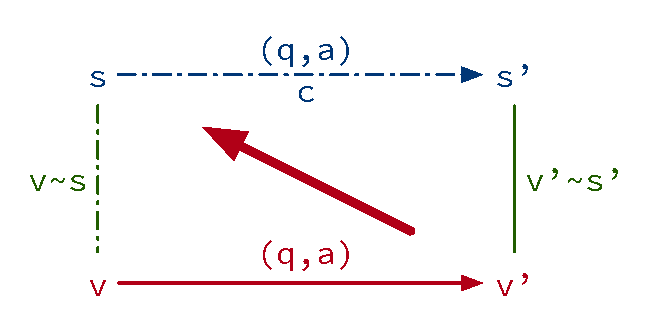
\includegraphics[width=.5\textwidth]{figures/complete}
  \end{center}

\item The initial validator state only reflects the initial server state:
  \begin{equation}
    \tag{RejComplete3}
    \label{eq:rc3}
    \{s\mid\Reflects{v_0}{s}\}=\{s_0\}
  \end{equation}
\end{enumerate}

Rejection soundness is proven by forward induction, while rejection completeness
is proven by backward induction.  This is because the choice $c$ is known from
the server step, while unknown from the validator step: Given a validator step,
we cannot predict ``what choices the server will make in the future'', but can
analyze ``what choices the server might have made in the past''.  This proof
method is further explained with the $\Prog$ example:

For specifications written in the $\Prog$ language, the server state is a
mapping from addresses to data; the validation state is a mapping from addresses
to symbolic variables, and constraints over the variables.  A validation state
is accepting if its constraints are satisfiable, {\it i.e.}  there exists an
{\em assignment} of the symbolic variables that can unify the trace with the
server model.  The internal choices made by the server are represented as
symbolic variables.  The assignment maps these variables to the choices' value
at each step, from which we can reconstruct the server's execution path.
\begin{definition}[Bisimulation for $\Prog$ specifications]
  Validator state $v$ {\em simulates} server state $s$ if it contains a
  validation state $(vs,cs)$ that {\em reflects} the server state: (1) There
  exists an assignment $asgn$ that can satisfy the constraints $cs$; and (2) The
  address-variable mapping $vs$ can be {\em instantiated} with the assignment
  (written as ``$vs^{asgn}$'') into an address-data mapping that is equivalent
  with $s$:
  \begin{align*}
    \Reflects v s\quad\triangleq\quad& \exists((vs,cs)\in v)(asgn:\Nat\to\Nat),\satisfy{asgn}
    cs\wedge vs^{asgn}=s\\ vs^{asgn}\quad\triangleq\quad&addr\mapsto
    asgn!(vs!addr)
  \end{align*}
\end{definition}
This bisimulation definition satisfies the hypotheses for proving soundness and
completeness:

Hypotheses~\ref{eq:rs1} and \ref{eq:rc3} are immediate from the initial states'
definition: The initial server state is all-zero map.  The initial validator
state is a singleton that maps all addresses to a variable that is constrained
to have value zero.

\autoref{eq:rc1} is based on the fact that $\vstep_p$ checks the nonemptiness of
the result:
\[\forall q~a~v~v',\vstep_p(q,a,v)=\Some{v'}\implies(\vstep_p'(q,a,v)=v'\wedge\exists (vs,cs)\in v')\]
and that $\vstep_p'$ guards the satisfiability of all constraints in its result:
\[\forall q~a~vs~cs,{(vs,cs)}\in\vstep_p'(q,a,v)\implies\exists asgn,\satisfy{asgn}cs\]

Therefore, any element in the resulting validator state can construct a
simulating server state:
\[\forall asgn~cs~vs~v,(\satisfy{asgn}cs\wedge(vs,cs)\in v)\implies \Reflects{v}{vs^{asgn}}\]

\autoref{eq:rs2} is based on the fact that the pre-validation state must contain
an element that reflects the server's pre-execution state, as defined by the
bisimulation relation.  Given the server's internal choices, we can compute its
execution path.  By induction on the server's execution path, we can construct
the corresponding post-validation state by making the same internal choice and
branch decisions as the server did, and construct the assignment that satisfies
the validator's constraints.

\autoref{eq:rc3} observes that validator design increases the constraints
monotonically.  Therefore, ``assignments that can satisfy the post-validation
constraints'' is a subset of ``assignments that can satisfy the pre-validation
constraints'':
\[\forall q~a~vs~cs~vs'~cs'~asgn,((vs',cs')\in\vstep_p'(q,a,(vs,cs))\wedge\satisfy{asgn} cs')\implies\satisfy{asgn}cs\]

As a result, the corresponding pre-step server state and the internal choice can
be constructed, and proven to perform the server-side step:
\begin{align*}
\forall q~a~vs~cs~vs'~cs'~asgn,\;&(vs',cs')\in\vstep_p'(q,a,(vs,cs))\\
&\implies\sstep_p(q,asgn!(\Fresh{vs}),vs^{asgn})=vs'^{~asgn}
\end{align*}

The intuition here is that the assignment includes ``all choices made by the
server, past and future'', which is narrowed upon more and more observations.
Therefore, the assignment can instantiate all previous validator states into
corresponding servers, and reconstruct the server's execution path by inferring
its internal choices.
